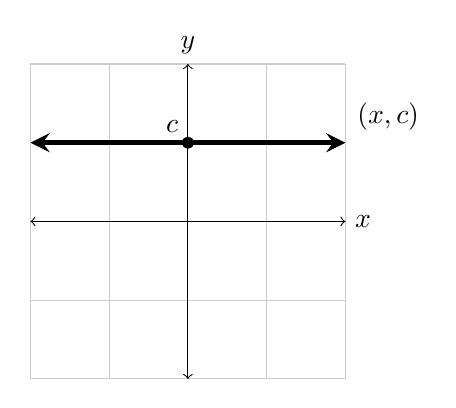
\begin{tikzpicture}
    \draw[thin,gray!40] (-2,-2) grid (2,2);
    \draw[<->] (-2,0)--(2,0) node[right] {$x$};
    \draw[<->] (0,-2)--(0,2) node[above]{$y$};
    \draw[fill=black] (0,1) circle(2pt) node[anchor=south east]{$c$};
    \draw[line width=2pt,black,stealth-stealth] (-2,1)--(2,1) node[anchor=south west]{$(x,c)$};
\end{tikzpicture}
\caption*{Linea horizontal real}